\documentclass[sigconf,nonacm,10pt]{acmart}
\settopmatter{printacmref=false,printfolios=true}
\setcopyright{none}
\renewcommand\footnotetextcopyrightpermission[1]{}
\usepackage{amsmath,tabularx,array,enumitem,balance,tikz,xurl}
\geometry{a4paper,left=15mm,right=15mm,top=15mm,bottom=15mm}
\usetikzlibrary{arrows.meta,positioning}
\definecolor{CourseBlue}{HTML}{315EFB}
\definecolor{CourseTeal}{HTML}{14877D}
\definecolor{CourseInk}{HTML}{18324A}
\hypersetup{colorlinks=true,linkcolor=CourseBlue,citecolor=CourseTeal,urlcolor=CourseTeal}
\newcolumntype{Y}{>{\raggedright\arraybackslash}X}
\setlist{leftmargin=*,topsep=2pt,itemsep=1pt}
\setlength{\emergencystretch}{2em}

\title{Compute Commons: Usable Access to Robot Inference}
\author{Xinrong Sun}
\affiliation{\institution{Duke Kunshan University}\city{Kunshan}\country{China}}
\email{xs156@duke.edu}
\renewcommand{\shortauthors}{Xinrong Sun, FP9}
\begin{document}
\begin{teaserfigure}
\centering
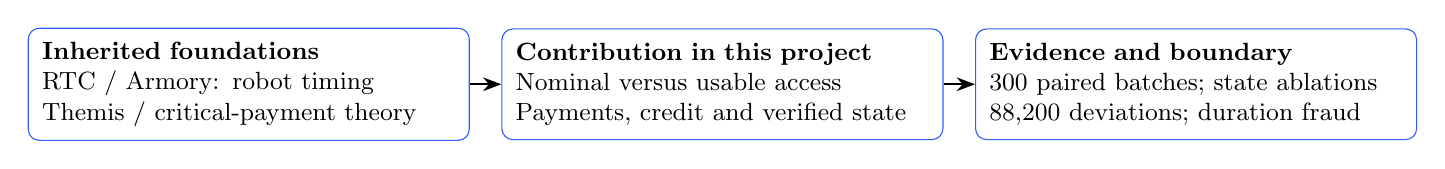
\begin{tikzpicture}[n/.style={draw=CourseBlue,rounded corners,align=left,font=\small,text width=5.25cm,minimum height=1.05cm,inner sep=5pt},>=Stealth]
\node[n] (a) {\textbf{Inherited foundations}\\RTC / Armory: robot timing\\Themis / critical-payment theory};
\node[n,right=0.4cm of a] (b) {\textbf{Contribution in this project}\\Nominal versus usable access\\Payments, credit and verified state};
\node[n,right=0.4cm of b] (c) {\textbf{Evidence and boundary}\\300 paired batches; state ablations\\88,200 deviations; duration fraud};
\draw[->,thick] (a)--(b);\draw[->,thick] (b)--(c);
\end{tikzpicture}

\caption{Inherited foundations, project contribution and evidence. Public robot constraints define usable allocations; the final self-test separates deadline reports from execution-time manipulation. All numerical evidence is synthetic.}
\label{fig:teaser}\Description{Three linked blocks: foundations, usable-access mechanism, and reproducible tests.}
\end{teaserfigure}
\maketitle\raggedbottom
\noindent\textbf{COMSCI/ECON 206: Computational Microeconomics.} Autumn 2026 Session 1. Instructor: Professor Luyao Zhang. \textbf{FP9: Compute Commons.} Solo final project, October 21, 2026.

\section{Background}
A robot may win inference time yet receive no usable result: its action queue can expire, or a moving target can leave the allowed pose tolerance. RTC studies delayed action execution \cite{rtc}; Armory studies heterogeneous robot policy serving \cite{armory}; Themis already links GPU allocation and fairness \cite{themis}. Our gap is a bounded comparison of usable service, private-value incentives and access policies, not the invention of deadline-aware scheduling.

\section{Motivation}
Charging for an expired result changes the incentive to participate. A nominal allocation therefore cannot stand in for usable access. The policy decision is how to distribute timely service and disclose the value cost of entrant priority and worker evaluation reserves.

\section{Application Scenario}
Independent small integrators and incumbent operators share a tabletop pick-and-place inference server. A coordinator commits to admission and payments; workers select tasks for reserved evaluation time. Verified telemetry fixes physical feasibility. Local fallback and protective control lie outside the auction; timely inference does not certify robot safety.

\section{Research Question}
\textbf{Shared question:} Can an access policy allocate usable robot inference while preserving truthful value reports? \textbf{Economics:} how do task value and entrant access trade off? \textbf{Computation:} which state constraints and reports change outcomes? \textbf{Behavior:} can users distinguish payment from timely completion? The final self-challenge tests the boundary between verifiable state and strategic reports.

\section{Method}
All jobs arrive at time zero at one nonpreemptive server. Operator $i$ privately values a timely result at $v_i\geq0$ and submits a sealed bid $b_i\geq0$. Public data specify service time, queued steps $h_i$, control period $\Delta_i$, pose tolerance $\epsilon_i$, speed bound $w_i$, network delay $\eta_i$ and guard time $g_i$. In milliseconds,
\[
d_i=\min\{h_i\Delta_i,1000\epsilon_i/w_i\}-\eta_i-g_i.
\]
For $w_i=0$, pose lifetime is infinite. Enumerate subsets, check earliest-deadline-first (EDF) completion against $d_i$ and horizon $T-r$, and maximize $\sum_i(b_i+ce_i)x_i$. Here $r$ reserves tail time and $e_i$ is verified entrant status. Winners pay $p_i=\max\{0,H_i^0-H_i^1-ce_i\}$, with best rival scores $H_i^0$ excluding $i$ and $H_i^1$ feasible with $i$. Losers pay zero; a fixed tie rule applies. Execution and settlement end the round.

\textbf{Game theory:} utility is $v_i$ for timely delivery minus payment. Fixed public feasibility gives dominant-strategy truthful values and a truthful Bayesian equilibrium under any private-value prior \cite{roughgarden,harsanyi}. \textbf{Social choice:} report task value, revenue, usable entrant access and reserved time separately; credits express policy priority, not measured social benefit. \textbf{Mechanism design:} compare capacity-only admission, EDF without payments, feasible admission, credits and reserves. Capacity-only admission is a diagnostic, not a physical-equilibrium benchmark. Exact enumeration is an offline oracle limited to 12 jobs.

\section{Results}
\begin{center}\small\setlength{\tabcolsep}{4pt}
\begin{tabular}{lcccc}\toprule
Rule & Admit & Pays & Value & Rev.\\\midrule
Capacity only & $A,B$ & $8,8$ & 10 & 16\\
EDF & $A,D$ & $0,0$ & 18 & 0\\
Feasible & $A,D$ & $9,6$ & 18 & 15\\
Credit $c=3$ & $A,E$ & $9,5$ & 16 & 14\\
Reserve $r=100$ & $A$ & 9 & 10 & 9\\
Both $r=100,c=5$ & $E$ & 5 & 6 & 5\\\bottomrule
\end{tabular}\end{center}
\noindent\textbf{Worked synthetic batch:} $T=400$ ms, each job 200 ms, values $(10,9,8,6)$ and deadlines $(200,200,400,400)$ for $A,B,D,E$; only $E$ is eligible. Capacity-only $B$ pays 8 for a late result and gains by bidding zero. Removing either queue or pose constraint permits $A,B$ and value 19. Credit 3 buys entrant access at a two-unit value cost. Across 300 paired six-robot batches (seed 206), mean values are 21.30, 38.86 and 43.06 for capacity-only, EDF and feasible allocation; Appendix A gives Monte Carlo intervals and 36,289 checks.

\textbf{Final self-test:} 88,200 joint bid/deadline deviations in 300 three-robot batches produce no positive gain. Appendix G explains the conditional result. In contrast, understating service time from 200 to 100 ms increases one operator's utility from 2 to 10. Verification must distinguish kinds of telemetry. The interface asks users to predict payment and timeliness separately before feedback \cite{hassidim}. Classroom questions motivate the test; automated interactions are not human-study evidence.

\balance
\section{Intellectual Merits}
RTC improves action continuity; Armory dynamically batches requests; Themis balances GPU efficiency and finish-time fairness. We do not reproduce or outperform those systems. Figure~\ref{fig:teaser} separates these foundations from our strategic counterexample, access trade-off and telemetry test. The critical-payment proof is established theory applied to this feasible family. Appendix G contains the three-paper comparison and expanded diagrams.

\section{Practical Impacts}
Operators could gain usable access and an appeal route for state errors. Academic evidence requires reproducibility; deployment requires calibrated latency and task success; public accountability requires transparent eligibility. The teaching artifact targets \textbf{SDG 4.4}: prediction accuracy before versus after a deadline explanation is the proposed indicator, not a measured benefit. Risks include exclusion through priority rules and confusing deadlines with safety. Publish access/value trade-offs and retain local safety control. The official-icon impact diagram is in Appendix G.

\subsection*{Future Research Roadmap}
Appendix G links the self-test to economics (audited duration reports), CS (matched Armory traces and solver overhead), and behavior (payment versus deadline explanations). Each study specifies data, a possible collaborator, a success criterion and a milestone. None is presented as completed robot or participant research.

\noindent\textbf{2056 aspiration.} Develop accountable access institutions whose incentives and physical benefits can be tested independently. The 2025 Economics Prize's innovation-and-growth foundation \cite{nobel2025} motivates studying who can use technological progress; our static model establishes no growth effect.

\noindent\textbf{Open artifacts.} \href{https://github.com/dku-comsci-econ206-Autumn2026/-PS2-FP9-ComputeCommons}{GitHub and embedded poster}; \href{https://huggingface.co/spaces/dku-comsci-econ206-2026/compute-commons}{Hugging Face}; \href{https://www.overleaf.com/project/6ac3a483f8fd778ea3fdc65f}{Overleaf}. Run \path{code/robot_model.py} and \path{code/deadline_test.py}. Release \texttt{final-fp9-2026-10-21}; tested source hashes and notebook are in the release record.

\clearpage\nobalance
\section*{Author Notes}
\subsection*{Full Acknowledgments}
We thank Prof. Luyao Zhang for the course framework, project guidance and templates; Prof. Kenneth S. (Ken) Rogerson for feedback on improving the mechanism; and Han Zhang for sharing his project and urging us to distinguish robot inference from ordinary CPU allocation. Yiqiao Liu introduced Armory, challenged the novelty claim and proposed an equal-workload comparison through Ed and oral feedback; she also advised on referencing prior work in class. Xuantong Fu (FP3) identified the false-eligibility gain and called for reproducible, consistent artifacts. Muhan Chen provided oral and handwritten feedback. Tencent's Shanghai office provided the industry field-learning setting; the Shanghai Science and Technology Museum provided inspiration; and the COMSCI/ECON 206 classroom community enabled presentations and discussion. We credit Python, JavaScript, the course/ACM templates and cited research. Codex assisted revision and verification, as disclosed in Appendix A.

\subsection*{Updated Team and Individual Contributions}
\textbf{Xinrong Sun, sole author.} Her intellectual decisions were to distinguish usable access from nominal compute, identify missing robotics specificity, and challenge the public-telemetry assumption. Outputs are the model and comparisons in Sections 5--6, the paper, interactive artifact and A0 poster. She confirmed full review and online verification of the earlier revision. The October 20 automated verification reruns the inherited model and adds the deadline/duration test. Her original research and critique connect the economic objective, computational feasible set and behavioral predictions. She retains final intellectual responsibility; automated tests do not constitute participant observations.
\bibliographystyle{ACM-Reference-Format}\bibliography{references}
\appendix
\section{Technical details and reproducibility}
\subsection{Physical model, units and scope}
Each independently operated robot requests one nonpreemptive inference job in a batch released at time zero. No cross-robot collision or task externality is modeled. While it waits, an existing queue executes for $h_i\Delta_i$ ms. With target speed bounded by $w_i$ mm/s and allowed displacement $\epsilon_i$ mm, a constant-bound surrogate permits $1000\epsilon_i/w_i$ ms of observation age. The minimum of these two times, minus network and guard time, is the server completion deadline. Jobs that cannot meet it take an assumed local fallback and obtain zero incremental task value. This is a model of admissible freshness, not a measured grasp-success function, a stability certificate, or a contact dynamics simulator.

OpenVLA motivates shared inference; no OpenVLA checkpoint was executed. RTC motivates the action-queue issue, but its algorithm is not reproduced. Our pose bound is a proposed simplifying assumption, not a theorem or measurement from either paper. Predictive tracking, refreshed observations, variable policy quality and common physical workspaces would change the valuation domain. The admission computation is offline: a deployment must include solver overhead in the time budget and measure worst-case or tail delays.

\begin{center}\small
\begin{tabularx}{\columnwidth}{lY}\toprule
Parameter & Worked instance / interpretation\\\midrule
$n,T,r$ & 4 jobs; 400 ms horizon; reserve 0 or 100 ms at its end.\\
$v$ & $(10,9,8,6)$ for $A,B,D,E$, synthetic private incremental values.\\
$e,c$ & $(0,0,0,1)$; credit 0, 3 or 5 in value units.\\
$\ell,\Delta$ & 200 ms per inference; 100 ms control period.\\
$h$ & $(2,4,4,4)$ queued control steps.\\
$\epsilon,w$ & $(20,10,20,20)$ mm tolerance; 50 mm/s speed for all.\\
$\eta,g$ & Both zero in the worked instance; network delay varied separately.\\
$d$ & $(200,200,400,400)$ ms.\\\bottomrule
\end{tabularx}
\end{center}
All values and telemetry are illustrative. All participants observe the rule and public state but only their own private value. A strategy maps value to one nonnegative sealed bid. A prior is unnecessary for dominant-strategy analysis; any prior over private values yields the stated truthful Bayesian equilibrium. Worker task selection and the coordinator's commitment are institutional assumptions, not additional solved games.

\subsection{Feasibility and incentive argument}
For a fixed subset with all release times zero and deterministic processing times, EDF detects feasibility: swapping an adjacent inverted-deadline pair cannot make either deadline harder to meet when the original order was feasible. Repeated exchanges yield EDF. This claim does not extend unchanged to release times, preemption constraints beyond this model, or sequence-dependent execution times.

Fix rivals' bids and public inputs. The best score among sets containing $i$ is $b_i+ce_i+H_i^1$; the best score excluding it is $H_i^0$. Both $H$ terms are independent of $b_i$. Thus the winning threshold is $H_i^0-H_i^1-ce_i$, subject to the fixed boundary tie rule. Truncate the threshold at zero because bids are nonnegative. Winning at the threshold price gives $v_i-p_i$; losing gives zero. Bidding one's value selects a nonnegative-utility outcome and no unilateral deviation improves it. If no feasible set contains $i$, every report loses. This proves value DSIC, ex-post individual rationality and nonnegative payments under the declared domain using standard critical-payment theory \cite{roughgarden}.

The fixed lexicographic tie rule favors inclusion of earlier bidder indices. Numerical verification does not replace the proof. Credit is a public score offset and creates no cash subsidy. With nonbinding deadlines and identical inference duration, the feasible family is a cardinality constraint and the mechanism reduces to the earlier unit-demand auction. With heterogeneous durations, it generalizes that benchmark to a capacity-constrained subset problem.

\subsection{A strategic counterexample to nominal service}
Capacity-only admission selects $A,B$ and charges 8 each in the worked instance. EDF dispatch gives $A$ completion 200 ms and $B$ completion 400 ms. Since $B$'s deadline is 200 ms, its realized utility is $-8$. Reporting zero removes $B$ and produces utility zero: truthful bidding is not an equilibrium of this diagnostic mechanism when values attach to timely output. Under feasible admission, $A,D$ pay 9 and 6 and obtain utilities 1 and 2. Credit 3 selects $A,E$, paying 9 and 5, each with utility 1. Reserve alone yields utility 1 for $A$; the combined treatment yields utility 1 for $E$. Losers pay zero in all rules.

There is no refund in the deliberately mismatched baseline. Adding contingent refunds defines a different mechanism requiring new incentive analysis. Likewise, physical-state falsification and false eligibility are outside the proof. The inherited model's false-label example remains reproducible in \texttt{code/model.py}; it is a distinct legacy experiment, not a result of the new robot model.

\textbf{Worked strategic representation.} Fix $D,E$ at bids 8 and 6 under the feasible rule, credit zero, and true values $v_A=10,v_B=9$. Restrict the displayed actions to zero and truthful bidding; entries are $(u_A,u_B)$:
\begin{center}\begin{tabular}{lcc}\toprule
 & $b_B=0$ & $b_B=9$\\\midrule
$b_A=0$ & $(0,0)$ & $(0,3)$\\
$b_A=10$ & $(4,0)$ & $(1,0)$\\\bottomrule
\end{tabular}\end{center}
The truthful pair is a Nash equilibrium in this displayed restriction. The earlier threshold argument, not this finite matrix, establishes the full private-type strategy result.

\subsection{Language-independent pseudocode}
\begin{enumerate}
\item Validate finite nonnegative inputs, positive service and control times, binary eligibility, and reserve no greater than horizon.
\item Convert robot state into server deadlines, using an infinite pose bound for a stationary target.
\item Enumerate subsets. Sort each by deadline, then index; accumulate execution time and reject any deadline or horizon violation.
\item Maximize credited bid sum over feasible subsets, resolving equal objectives using the fixed allocation order.
\item For each winner compute best rival score with and without that winner; charge its nonnegative critical value.
\item Evaluate actual completion against physical deadlines. Report value, utility, revenue, nominal/usable access, late jobs and wasted inference time.
\item Repeat with identical inputs for all mechanisms, and independently verify feasibility and unilateral deviations.
\end{enumerate}
The exponential oracle is deliberately limited to at most 12 jobs. Sorting/subset enumeration and repeated threshold scans give the upper bound of $O(2^n n\log n+n^2 2^n)$. No online scalability claim follows.

\subsection{Actual synthetic sweep and sensitivity}
\begin{center}\small\begin{tabular}{lrrrr}\toprule Rule & Value & Revenue & Entrant & Late\\\midrule
Generic & 21.30 & 14.29 & 0.55 & 2.92\\
EDF & 38.86 & 0.00 & 1.17 & 0.00\\
Feasible & 43.06 & 8.74 & 1.19 & 0.00\\
Credit 3 & 42.99 & 8.43 & 1.26 & 0.00\\
\bottomrule\end{tabular}\end{center}
Feasible minus generic: mean value difference 21.76, paired 95\% Monte Carlo interval [20.05, 23.46].
Feasible minus edf: mean value difference 4.20, paired 95\% Monte Carlo interval [3.50, 4.90].
The generator uses Python's seeded random number generator (seed 206), 300 paired instances, six robots and a 600 ms horizon. Values are discrete uniform integers 1--20. Service time is sampled uniformly from 50, 100, 150 and 200 ms; queue depth from 1--8; tolerance from 10, 20 and 40 mm; speed from 25, 50 and 100 mm/s; network delay from 0, 25 and 50 ms. These quantities are sampled independently. The last two indices are eligible. Credit is 3 and reserve is zero in the random comparison. No parameters were fitted to robot traces.

\begin{sloppypar}
The 95\% intervals are paired mean differences plus/minus $1.96$ standard errors across generated instances. They describe Monte Carlo variability under this arbitrary generator, not external validity or human evidence. Exact feasible optimization weakly dominates any feasible EDF allocation in raw value by construction at zero credit; the comparison measures the size of that modeled opportunity, not a surprising theorem. Revenue for the capacity-only rule includes late-result charges and must not be interpreted as acceptable deployed revenue.
\end{sloppypar}

In the worked ablation, removing queue expiry relaxes $A$ while $B$ remains urgent, and removing pose freshness relaxes $B$ while $A$ remains urgent. Either permits serving both. Removing both gives the generic-capacity special case. Added known network delay of 25 ms invalidates both 200 ms urgent jobs, so feasible admission falls to $D$ only, value 8. This discontinuity is an explicit failure of zero-slack calibration. Unknown execution-time error, variable motion and safety outcomes remain untested.

\subsection{Reproduction and AI-use record}
Run \texttt{python} \path{code/robot_model.py} with Python 3.10 or later (standard library only). It writes \texttt{robot\_results.json} and \texttt{robot\_sweep.csv} beside the source. The notebook embeds the same source for offline execution. \texttt{code/robot-fresh-run.txt} records actual execution. The old \texttt{model.py} and its outputs are retained as explicitly labeled legacy evidence.

\textbf{Assistance disclosure, October 5--21, 2026.} OpenAI Codex (GPT-6-based agent) supported revision of the author's existing project at her request: robotics literature checking, model refinement, code verification and artifact preparation. Incorporated suggestions concerned action-buffer and pose-freshness constraints, critical payments, baselines, ablations and behavioral questions. The author supplied the original project and robotics-specificity critique, directed the revision, and confirmed review and approval of the earlier revision. The October 20 request was to migrate to the supplied final template and added rubric. Accepted assistance includes the eight-part structure, native diagrams, reproducibility checks and a joint-report test. Rejected suggestions include treating red-team access as a completed new study, claiming Armory superiority, or inventing participant records. Computational checks are recorded above and in Appendix G. Xinrong Sun is the sole author and takes responsibility for all submitted content.

\section{Cumulative intellectual development}
\textbf{Earlier work (supplied source).} PS1 distinguished consultation from binding access. The supplied PS2 draft introduced private values, credits and reservations but explicitly excluded real-time control. Its numerical claims concern interchangeable windows. \textbf{October 5 critique (author).} Robot specificity was insufficient: changing the device label left the mechanism unchanged. \textbf{Revision.} State-derived deadlines now change feasible allocations; raw compute and usable access become distinct metrics. \textbf{Consequence.} The baseline's rationality diagnosis changes when nominal wins have no physical value. Prior files are preserved in the original project directory; this revision has its own source and results.

\section{Verified literature and three-lens checks}
\textbf{Armory \cite{armory}.} The closest multi-robot serving comparison uses dynamic batching and closed-loop execution. It permits task-dependent weights. This final revision narrows the contribution to incentives and access trade-offs; a matched Armory benchmark is future work, not an existing result.

\textbf{RTC \cite{rtc}.} Question: how to execute action chunks despite inference delay. Method: asynchronous chunk generation with inference-time conditioning. Evidence: simulated and real manipulation tasks. Its contribution concerns action continuity and delay robustness. Here, the auction allocates across operators and uses a simple public queue constraint. We neither reproduce RTC nor claim its latency-control insight as original.

\textbf{Deadline-aware task and motion planning \cite{sung}.} Question: how to distribute planning effort under uncertain planning/execution times. Method: an MDP, complexity analysis and approximate search. Evidence: computational experiments. This invalidates a broad novelty claim about deadline-aware robot computation. Our single-batch, deterministic, private-value mechanism instead studies payments and distributive access; the paper supplies no performance benchmark for our auction.

\textbf{FogROS2 \cite{fogros}.} Question: how to execute robot computations on cloud/fog resources. Method: ROS 2 integration and infrastructure selection. Evidence: robotic workloads with measured timing. This motivates measuring network and processing delay separately. Our assumed deterministic delays are not FogROS2 measurements.

\textbf{Themis \cite{themis}.} Question: fair GPU sharing for training workloads. Objective: finish-time fairness and efficiency. Method: auction-based scheduling sensitive to placement. Evidence: workload evaluation. It defeats a claim that fairness and compute auctions are new. Our public physical feasibility and usable entrant-access objective differ; we do not claim superior scheduling to Themis.

\textbf{Vickrey / Myerson framework \cite{vickrey,roughgarden}.} Supplies established incentive theory, not a novel contribution of this project. \textbf{OpenVLA \cite{openvla}.} Supplies application context and published robot-learning evidence; this revision has no trained-policy evaluation. \textbf{Behavior \cite{hassidim}.} Misreporting under strategy-proof matching motivates separating comprehension and beliefs. It does not establish the cause of behavior in our auction.

\textbf{Consequence check.} Game theory forces us to distinguish true timely-service utility from nominal allocation and provides a deviation test. Social choice forces separate usable-access and value metrics and exposes the credit cost. Mechanism design changes admission and payment together. Each affects the same inference decision.

\textbf{Sources and reuse.} Official links and identifiers are in the bibliography. Access date: October 5, 2026. New code implements the model directly and does not import robotics software. The included MIT license covers original code, not third-party course/ACM templates or scholarly works. Source publications were checked through their project, arXiv, publisher or author pages; the review is targeted, not exhaustive. Template notices remain intact. Literature comparison establishes a bounded application gap, not worldwide priority.

\section{Review response and revision record}

\textbf{Yiqiao Liu, final-week Ed and oral feedback (author-confirmed October 21).} Yiqiao Liu introduced Armory and challenged novelty beyond scheduling plus critical payments. \emph{Revise}: Sections 1 and 7, Figure 1 and Appendix C now compare RTC, Armory and Themis and limit novelty. \emph{Keep}: the physical allocation/payments connection survives. \emph{Reasoned disagreement}: throughput alone cannot assess private-value incentives; add realized value and entrant access, reporting payments separately. \emph{Investigate}: a matched dynamic-batching benchmark requires a common execution model; no Armory superiority is claimed. The author supplied the comment and confirmed its attribution; Ed record: \url{https://edstem.org/us/courses/102917/discussion/8381683?comment=19460483}. Responsible author: Xinrong Sun.

\textbf{October 14 author self-challenge.} Could a false deadline improve utility? \emph{Test and revise}, October 20: 88,200 finite deviations found no gain; Appendix G supplies the conditional argument and a service-duration counterexample with gain 8. This changes the claim from general suspicion of deadline reports to a specific verification boundary. Locations: Section 6, Appendix G, code/deadline\_test.py and the demonstration's self-test panel. Responsible author: Xinrong Sun.

\textbf{Instructor final rubric, supplied October 20.} \emph{Revise}: migrate five PS2 sections into the eight required parts; retain A--F and add G; create the impact and roadmap diagrams, official SDG icon, contribution and credit blocks, and repository poster preview. Verification: source compilation, page-count and poster-dimension checks, fresh-run outputs and package audit. Responsible author: Xinrong Sun.


\textbf{Xuantong Fu (FP3), supplied peer-feedback record.} The false-label example gives $A$ a gain of 4, challenging unconditional truthfulness; code results should reproduce across artifacts. \emph{Revise}: distinguish value reports from eligibility reports and state verified eligibility as a condition. The legacy profile $(10,9,6)$, reserve 1 and credit 5 changes $A$'s utility from 0 to 4 when it falsely claims eligibility. This is the earlier unit-window model, not the final duration test. \emph{Keep}: conditional value truthfulness; \emph{Investigate}: qualification auditing. Verification: rerun the legacy counterexample, retain robot and JavaScript parity checks, and identify the final release. Locations: Appendix A, \path{code/model.py}, \path{evidence/final-release.json}. Responsible author: Xinrong Sun.

\textbf{Han Zhang, discussion reported by the author.} Distinguish robot inference from an ordinary CPU auction. \emph{Revise}: action-buffer expiry and target-pose validity determine physical deadlines; relaxing either constraint changes the worked allocation. Verification: the two state ablations in \path{code/robot_results.json}. Locations: Sections 1, 3, 5--6 and Appendix A. Responsible author: Xinrong Sun.

\textbf{Prof. Ken Rogerson and Muhan Chen.} The author reports that Prof. Rogerson offered mechanism-improvement feedback, while Muhan Chen supplied oral and handwritten suggestions. Their contributions are credited without attributing an unrecorded specific proposition to them. The final mechanism, limits and response record make the resulting project available for their review. The author's acknowledgment post is \url{https://edstem.org/us/courses/102917/discussion/8381683?comment=19460597}.

\textbf{Revise: author's October 5 comment.} The robot label was interchangeable with generic compute. Changed Sections 1--3, the model, experiment, interface and poster to include queue expiry and pose freshness. Verification: worked counterexample, two channel ablations, EDF comparator and finite incentive tests.

\textbf{Keep: original access question.} Retained entrant priority and worker evaluation rights, but defined the reserve in milliseconds and measured entrant access after physical usability. Cost is reported instead of describing rights as automatically welfare-improving.

\textbf{Investigate: international publication.} Requires calibrated robotics workloads, independent baselines, online compute overhead, actual robot success/fallback measures and a literature search sufficient for the target venue. Synthetic examples alone are insufficient.

\textbf{Submission verification.} Xinrong Sun confirmed online verification and approval of the earlier revision. The October 20 release records the subsequent computational checks separately.

\clearpage\onecolumn
\section{Structured abstract and cumulative proposal map}
\begin{table}[h]\small
\begin{tabularx}{\textwidth}{p{0.20\textwidth}Y}\toprule
Element & Current statement\\\midrule
Background & Interchangeable compute rights may fail to provide timely robot actions. Existing scheduling, robotics and incentive theory establish the foundations.\\
Motivation and application & Shared tabletop pick-and-place inference for incumbent and small integrators, with worker-selected evaluation capacity.\\
Connected questions & How do usable access, value and revenue trade off; which physical constraints change allocation; and do people understand timely service and payments separately?\\
Methods and assumptions & Sealed private values, fixed public telemetry and eligibility, deterministic batch scheduling, exact subset maximization and critical payments. Compare generic admission, EDF, feasible auction and access policies.\\
Actual / planned results & Actual synthetic worked value is 10 for generic admission, 18 for feasible admission and 16 with credit 3. Code executes 300 paired instances and 36,289 checks. Robot trials and human pilot remain planned.\\
Intellectual merit & A nominal allocation can defeat both the access objective and the intended value incentive. Public physical feasibility restores the stated incentive domain under a bounded model.\\
Practical impact & Potentially usable access with transparent value costs. Needs verified telemetry, local fallback and an appeal route. No safety, educational or population benefit is established.\\
Feedback and revision & Author's October 5 specificity critique changes the feasible set, metrics and behavioral diagnosis. Earlier files remain available. The author confirmed review of the earlier revision; the final release records the subsequent October 20 computations.\\\bottomrule
\end{tabularx}
\caption{The same research question and evidence boundary across all revised artifacts.}
\end{table}
\clearpage\twocolumn
\section{PS2 extension: auction and artifact record}
\subsection{Auction laboratory}
Game identifier: \texttt{compute-commons-robot-v2}. The synthetic laboratory uses the four robot states in Appendix A, truthful algorithmic bids $(10,9,8,6)$, fixed index order $A,B,D,E$, and the six treatments in the main-text results table. Actual results include all payments, utilities, completion times and expiry flags in \texttt{robot\_results.json}. Prediction: truthfulness only for the physically feasible critical-payment rules. The generic diagnostic violates that prediction through negative realized utility. EDF is a nonmarket baseline; its zero payments are not auction revenue evidence.

The interface requires prediction before feedback and allows a facilitator to enter peer bids collected privately beforehand. Local JSON records contain treatment, public inputs, predictions, confidence, own bid, outcome and reflection. No personal names are necessary; no automatic response upload occurs. Synthetic opponents, manual entries and completed human observations must remain distinct. No human dataset accompanies this revision; valid completed-interaction count in the supplied evidence is zero.

\subsection{Artifact parity and release}
The Python oracle, notebook, JavaScript interaction, paper and poster use the same worked profile. The source package retains older evidence clearly labeled as legacy. The formal submission destinations are \url{https://github.com/dku-comsci-econ206-Autumn2026/-PS2-FP9-ComputeCommons} and \url{https://huggingface.co/spaces/dku-comsci-econ206-2026/compute-commons}. The supplied text entry names prior commit \texttt{b03cac82a1b535aa8dbcbd7f1608905386ec5f93}; it must not be represented as containing this revision. Current revision commit and publication status are recorded in the delivered release manifest and text entry.

\subsection{Practical-impact and final-review record}
The final submission is dated October 21, 2026; earlier PS2 sources are preserved. New computations are dated when executed and do not represent October 12--14 classroom observations. A prospective deployment would allow workers to contest unused reservations and operators to appeal telemetry or eligibility errors. The empirical falsifier is whether measured usable-action rates and value tradeoffs agree with the deadline surrogate under calibrated workloads.

\textbf{Human responsibility.} The research direction and original project are Xinrong Sun's. The author retains responsibility for every submitted claim and artifact. She confirmed review of the earlier manuscript and artifacts and directed this final-template revision. Her original research question and critique guide the changes.

\clearpage\onecolumn
\section{Final Week Evidence and Final Release Audit}
\subsection{Self-challenge: deadline reports and execution time}
\textbf{Question, Xinrong Sun, October 14.} Can an operator improve her payoff by reporting false deadline information? The original value-DSIC proof fixes telemetry. The final computation therefore evaluates joint changes in value bids and reported deadlines while computing utility from actual deadlines. It uses 300 seeded three-robot batches, bids 0--13, reported deadlines 1--7, service times 1 or 2, true values 1--12, true deadlines 1--6, horizon 6 and credit 0 or 2. All 88,200 deviations have gain at most zero. Units here are normalized time units. The finite test is a diagnostic, not a general theorem.

\textbf{Conditional argument.} Fix truthful rivals, verified durations and eligibility. Let $H^0$ be the best rival score without $i$ and $H^1(d)$ the best rival score in a feasible set containing $i$ with its true deadline $d$. The honest critical price is $p=\max(0,H^0-H^1(d)-ce_i)$. Consider any bid/deadline deviation. Losing yields zero. A winner finishing after its true deadline has utility $-p'\leq0$. If a deviating winner finishes on time, the selected schedule is also feasible with its true deadline; its rivals' score equals the reported conditional optimum $H^1(\hat d)$ because the bidder's own score is constant across all sets containing it. Thus $H^1(\hat d)\leq H^1(d)$ and $p'\geq p$. If honest reporting wins, the deviation cannot improve its utility; if honest reporting loses, $v_i\leq p$ (including ties), so the deviation cannot give positive utility. This extends the threshold reasoning only to an operator's own deadline and bid, under exact allocation, fixed other feasibility data and nonrefundable charges for late service. It is not a new general scheduling theorem or a guarantee for arbitrary telemetry.

\textbf{Duration counterexample.} Three jobs $A,B,C$ have values $(10,9,8)$, actual service times $(200,100,100)$ ms and deadlines 300 ms; the horizon is 300 ms and credits are zero. Honest allocation chooses $A,B$, with $A$ paying 8 and receiving utility 2. If $A$ reports 100 ms, the mechanism admits all three and charges $A$ zero. Real execution in the reported EDF/index order finishes at $(200,300,400)$ ms. $A$ is timely and gains 8 utility units; $C$ is late. Public execution-time verification is consequential. The implementation records reported allocation and actual execution separately, avoiding the mistake of evaluating physical utility using the false report.

\subsection{Intellectual Merits: annotated research/model diagram}
\begin{figure}[h]\centering
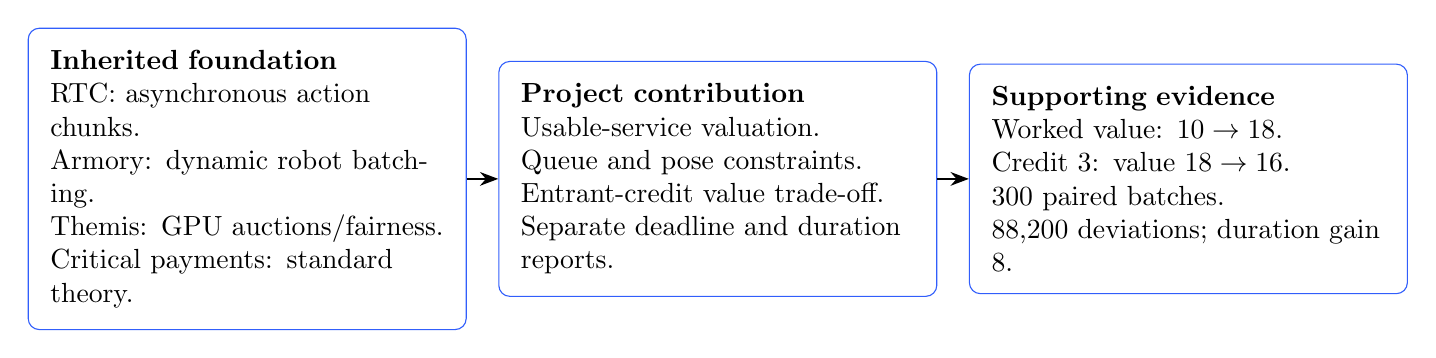
\begin{tikzpicture}[n/.style={draw=CourseBlue,rounded corners,align=left,text width=5.0cm,minimum height=2.6cm,inner sep=8pt},>=Stealth]
\node[n] (a) {\textbf{Inherited foundation}\\RTC: asynchronous action chunks.\\Armory: dynamic robot batching.\\Themis: GPU auctions/fairness.\\Critical payments: standard theory.};
\node[n,right=0.4cm of a] (b) {\textbf{Project contribution}\\Usable-service valuation.\\Queue and pose constraints.\\Entrant-credit value trade-off.\\Separate deadline and duration reports.};
\node[n,right=0.4cm of b] (c) {\textbf{Supporting evidence}\\Worked value: $10\to18$.\\Credit 3: value $18\to16$.\\300 paired batches.\\88,200 deviations; duration gain 8.};
\draw[->,thick] (a)--(b);\draw[->,thick] (b)--(c);
\end{tikzpicture}
\caption{The inherited algorithms are not reproduced; arrows indicate conceptual dependence, not performance superiority. All project outcomes are synthetic.}
\end{figure}
\small
\noindent\begin{tabularx}{\textwidth}{p{.15\textwidth}YYY}\toprule
Closest work & Method and objective & Evidence in that work & Difference and boundary here\\\midrule
RTC & Asynchronous chunk execution; delay robustness & Simulation and robot manipulation & We allocate among private-value operators; no policy-level comparison.\\
Armory & Closed-loop batching; executed robot time with optional weights & Simulated and real robot fleets & We study payment incentives and usable entrant access in a static abstraction. A common dynamic benchmark is future work.\\
Themis & Auction-based GPU allocation; finish-time fairness & ML workload evaluation & Our feasibility depends on robot state; access is measured after timely delivery. No broad compute-auction novelty.\\\bottomrule
\end{tabularx}
\normalsize
\paragraph{References for the diagram.}
Kevin Black, Manuel Y. Galliker and Sergey Levine (2025). \emph{Real-Time Execution of Action Chunking Flow Policies}. NeurIPS 2025. \url{https://doi.org/10.48550/arXiv.2506.07339}.
Rohan Bansal, David He, Nadun Ranawaka Arachchige, Zhenyang Chen, Soobum Kim, Kexin Rong and Danfei Xu (2026). \emph{Action Chunk Scheduling for Batched Robot Policy Serving}. \url{https://doi.org/10.48550/arXiv.2608.00337}.
Kshiteej Mahajan, Arjun Balasubramanian, Arjun Singhvi, Shivaram Venkataraman, Aditya Akella, Amar Phanishayee and Shuchi Chawla (2020). \emph{Themis: Fair and Efficient GPU Cluster Scheduling}. NSDI, 289--304. \url{https://www.usenix.org/conference/nsdi20/presentation/mahajan}.

\clearpage
\subsection{Practical Impacts: mechanisms, indicators and safeguards}
\begin{figure}[h]\centering
\begin{tikzpicture}[n/.style={draw=CourseTeal,rounded corners,align=left,text width=4.95cm,minimum height=2.5cm,inner sep=9pt},>=Stealth]
\node[n] (a) {\textbf{Institutional mechanism}\\Verified feasible admission\\Transparent entrant credits\\Publish value/access trade-offs};
\node[n,right=0.5cm of a] (b) {\textbf{Affected stakeholders}\\Small integrators and operators\\Workers selecting evaluation tasks\\Learners using the demonstration};
\node[n,right=0.5cm of b] (c) {
\includegraphics[width=1.2cm]{images/sdg4.png}\quad\textbf{Target 4.4}\\Technical learning: predict payments and timely completion before and after explanation.};
\draw[->,thick] (a)--(b);\draw[->,thick] (b)--(c);
\end{tikzpicture}
\caption{Intended impact pathway. Operational outcomes are synthetic; the educational link is a proposed test. SDG icon is an official UN asset, not a certification or endorsement.}
\end{figure}
\noindent\begin{tabularx}{\textwidth}{p{.18\textwidth}YYY}\toprule
Outcome & Indicator and baseline & Evidence & Risk and safeguard\\\midrule
Usable service & Timely jobs and task value versus capacity-only and EDF & Worked batch and 300 synthetic batches & Deadlines do not ensure safety; retain protective control and calibrate traces.\\
Entrant access & Eligible entrants completing on time; compare credit 0 and 3 & Worked credit changes winner $D$ to $E$, value 18 to 16 & Favoritism and efficiency loss; disclose eligibility, publish trade-offs, permit correction.\\
Worker authority & Reserved ms and actual worker-selected completed evaluations & Time reservation modeled; benefit not measured & Idle reserves or displaced service; log use and provide an appeal route.\\
SDG 4.4 learning & Payment error and completion-prediction accuracy before/after instruction, versus payment-only tutorial & Testable proposed indicator; no human effect estimate & Confusing winning with safe success; explicit task boundary and comprehension questions.\\\bottomrule
\end{tabularx}
\paragraph{Standards and accountability.} Academic evaluation requires reproducible claims and matched baselines. Industry deployment requires end-to-end latency, task-success and solver-overhead measurements. Public institutions require transparent access criteria and opportunities to challenge and correct errors. These standards complement rather than substitute for one another. No voting result is claimed: selecting a worker task is an assumed governance right, not an analyzed voting game.
\paragraph{Sources.} United Nations (2026), \emph{Goal 4: Quality Education}, Target 4.4, \url{https://sdgs.un.org/goals/goal4}; official icon from \url{https://www.un.org/sustainabledevelopment/news/communications-material/}. Avinatan Hassidim, D\'eborah Marciano, Assaf Romm and Ran I. Shorrer (2017), \emph{The Mechanism Is Truthful, Why Aren't You?}, AER 107(5), 220--224, \url{https://doi.org/10.1257/aer.p20171027}. Behavioral interpretation is motivated by this literature; its findings are not observations of this project.
\smallskip\noindent\small The content of this publication has not been approved by the United Nations and does not reflect the views of the United Nations or its officials or Member States.\normalsize

\subsection{Future Research Roadmap: a discriminating next study}
\begin{figure}[h]\centering
\begin{tikzpicture}[n/.style={draw=CourseBlue,align=left,text width=4.95cm,minimum height=1.6cm,inner sep=8pt},>=Stealth]
\node[draw=CourseTeal,align=center,text width=16.8cm,inner sep=7pt] (q) {\textbf{Current boundary: deadline-only reports survive the stated test; private duration can gain 8.}\\Which verification rule preserves incentives without excluding small operators?};
\node[n,below=0.6cm of q,xshift=-5.8cm] (e) {\textbf{Economics}\\Audit duration reports and bound profitable deviations.};
\node[n,right=0.35cm of e] (c) {\textbf{Computer science}\\Replay matched workloads; include batching and solver latency.};
\node[n,right=0.35cm of c] (b) {\textbf{Behavioral science}\\
\includegraphics[width=.65cm]{images/sdg4.png}\quad\textbf{4.4}: test explanations and prediction accuracy.};
\draw[->] (q.south)--(e.north);\draw[->] (q.south)--(c.north);\draw[->] (q.south)--(b.north);
\end{tikzpicture}
\caption{New final-project roadmap. Branches specify complementary tests; none represents completed deployment or a causal human-study finding.}
\end{figure}

\clearpage
\noindent\begin{tabularx}{\textwidth}{p{.13\textwidth}YYYY}\toprule
Study & Question and method/data & Possible collaborator & Progress criterion & Milestone\\\midrule
Economics & Can audited execution time deter joint reports? Exact small-instance enumeration, bounded penalty and audit-cost sensitivity. & Mechanism-design mentor; no collaboration claimed & Identify a violation or prove a stated incentive domain; report access cost & Reproducible counterexample suite and candidate audit rule before scaling.\\
Computer science & Does economic allocation add value beyond scheduling? Common simulator with Armory-style batching, fixed workloads and actual solver runtime. & Robotics serving researcher; invitation proposed & Compare timely completion, task value and entrant access at equal resource budgets & First reproduce each baseline on a matched static case; then add dynamics.\\
Behavioral science & Does explaining deadlines improve comprehension? Counterbalanced payment-only versus deadline-aware tutorial; anonymous consented responses. & FP10 Yiqiao Liu if interested; behavioral mentor & Payment error, timely-prediction accuracy and uncertainty; separate legitimacy & Preregister questions and analysis before a consented pilot; SDG 4.4.\\\bottomrule
\end{tabularx}
\paragraph{How the duet informs the roadmap.} The supplied pairing connects FP9's usable robot service to FP10's strategic drone disclosure. The shared issue is whether accurate information and digital access lead to useful physical outcomes. This motivates verifying both the content and timing of reports. The Armory critique specifically motivates the common-workload branch. The author confirmed on October 21 that Yiqiao Liu supplied the Armory critique; her Ed permalink is retained in Appendix D.
\paragraph{Roadmap references.} Bansal et al. (2026), \emph{Action Chunk Scheduling for Batched Robot Policy Serving}, full reference above, \url{https://doi.org/10.48550/arXiv.2608.00337}; Tim Roughgarden (2013), \emph{Algorithmic Game Theory, Lecture 3: Myerson's Lemma}, Stanford CS364A, \url{https://timroughgarden.org/f13/l/l3.pdf}; Hassidim et al. (2017), full reference on the impact diagram page, \url{https://doi.org/10.1257/aer.p20171027}.

\subsection{Dated intellectual development and available activity evidence}
\noindent\begin{tabularx}{\textwidth}{p{.14\textwidth}YY}\toprule
Date/stage & Record used in this revision & Consequence\\\midrule
PS1 / PS2 & Earlier proposal, auction code, payments and reserved evaluation time & Preserve the access question and earlier artifacts; distinguish old model outputs from robot results.\\
October 5 & Author's explicit critique that generic CPU allocation did not capture robotics & Queue/pose constraints change feasible sets and the interpretation of utility.\\
October 12 & Beginning-post draft, supplied FP9--FP10 pairing, Armory reviewer excerpt and written defense in the project discussion & Compare three close papers; state no Armory superiority; propose equal-workload evaluation.\\
October 14 & Xinrong Sun's self-challenge text: can a reported deadline change utility? & October 20 computation tests joint reports; retain a negative result and redirect to execution-time verification.\\
October 15 & Research-direction discussion about audited model access & Kept as future exploration; not inserted as completed foundation-model research.\\
October 20 & Final rubric, fresh computations, migrated sources and new diagrams & Eight named parts, Appendix G, synchronized model outputs and a traceable final package.\\\bottomrule
\end{tabularx}
\paragraph{First-hand reflection and behavioral boundary.} The author's own October 14 question expected a possible profitable false deadline. The finite test and conditional argument challenge that expectation and make the next test more precise. This is an author self-reflection, not an independently observed classroom sample. The interaction separates predicted payments, predicted timeliness, confidence and explanation; the distinction follows from the economic counterexample. Original peer-play response files, daily takeaway sheets and handwritten exits are not reconstructed from automated tests.
\paragraph{Recognition and interview.} A proposed citation for FP10 is: ``Privacy--Coordination Trade-off Award: for making confidentiality and useful drone coordination an explicit strategic question.'' Proposed support is a joint information-delay sensitivity test. This is the retained award draft, not evidence of an issued certificate or completed interview. The evidence index links the supplied Ed comments and distinguishes them from award and interview drafts.
\paragraph{2056 revision and Nobel foundation.} The 2025 official announcement recognizes Joel Mokyr, Philippe Aghion and Peter Howitt for explaining innovation-driven growth. This motivates asking whether institutions make technological progress accessible; it does not validate this auction or establish growth effects. The author's 2056 aspiration has narrowed from general participation to independently testable incentives and usable access. The 2026 award to Robert E. Hall and Michael Woodford recognizes the microeconomic foundations of macroeconomic stabilization \cite{nobel2026,aea2026}. Compared with the 2025 emphasis on innovation-driven growth, it motivates specifying individual incentives and expectations before making institutional claims. Our proposed extension therefore models repeated access, uncertain service time and expectations about verification. This is a methodological connection, not a contribution to macroeconomic stabilization; no growth or stabilization effect is established here.
\paragraph{Source for 2025 comparison.} Royal Swedish Academy of Sciences (2025), \emph{The Prize in Economic Sciences 2025: Press Release}, \url{https://www.nobelprize.org/uploads/2025/10/press-economicsciences2025-1.pdf}.

\subsection{Final release audit and record locations}
Release identifier: \texttt{final-fp9-2026-10-21}. Exact code checksums, tested commits and packaging records accompany \path{evidence/final-release.json}. Run \path{code/robot_model.py}, \path{code/deadline_test.py} and \path{verify-robot.cjs}. The notebook embeds the tested robot model and adds the final challenge. Browser fallback images are under \path{evidence/}. The poster preview, PDF and editable PPTX are under \path{poster/}; the root README embeds the preview and links the PDF. Main-paper results, the worked browser profile and the poster table share the same values and deadlines. The challenge panel displays the separate three-job duration test explicitly.

The formal team repository is \url{https://github.com/dku-comsci-econ206-Autumn2026/-PS2-FP9-ComputeCommons}; the demonstration destination is \url{https://huggingface.co/spaces/dku-comsci-econ206-2026/compute-commons}; the team Overleaf project is \url{https://www.overleaf.com/project/6ac3a483f8fd778ea3fdc65f}. Publication checks for this release are recorded with their actual outcomes, separately from the author's earlier confirmation. The final-week source index preserves the distinction between drafted posts and original posted records. New human observations, reviewer identities or classroom exchanges are not inferred from missing attachments.


\end{document}

